
\section{Complexidade}

O problema \rcsp\ � NP-dif�cil mesmo para o caso em que existe apenas um
�nico recurso (\cite{HZ80} \cite{GJ79}). N�s podemos reduzir um problema 
NP-dif�cil bem conhecido a ele, o {\bf problema da mochila} ({\it knapsack}), 
definido a seguir.

\begin{problema}{\textsc{Mochila}(N,w,v,d)}
Como par�metros do problema s�o dados:
\begin{itemize}
\item\ Um conjunto de itens $N = \{1, \dots, n\}$,
\item\ pesos $w_i \in \mathbb{N}$, $i = 1, \dots, n$, para esses itens,
\item\ valores $v_i \in \mathbb{N}$, $i = 1, \dots, n$, para esse itens,
\item\ um peso limite $d \in \mathbb{N}_0$.
\end{itemize}
O peso de um subconjunto $I \subseteq N$ �
$w(I) = \sum_{i \in I}{w_i}$, e seu valor � 
$v(I) = \sum_{i \in I}{v_i}$. O problema \textsc{Mochila} consiste em
encontrar um subconjunto de itens com valor m�ximo, cujo peso n�o excede
o limite $d$.
\end{problema}

\begin{teorema}{} O \rcsp\ � NP-dif�cil.
\end{teorema}

\begin{prova} A prova se d� pela redu��o do problema \mochila\ ao \rcsp.
Vamos tomar uma inst�ncia $I$ do problema \mochila. N�s podemos
construir uma inst�ncia $I'$ para o \rcsp\ como se segue:
\begin{itemize}
\item $V := N \cup \{0\}$.
\item $A := A_1 \cup A_2$.
    \begin{itemize}
        \item $A_1 := \{(i-1,i): i=1,\dots,n\}$,
        \item $A_2 := \{(i-1,i): i=1,\dots,n\}$.
    \end{itemize}
\item $s := 0$, $t := n$.
\item $k = 1$.
\item $l := d$.
\item 
$
	r_a := \left\{
	\begin{array}{ll}
		\begin{array}{ll}
			w_i, & \text{se } a \in A_1, \\
			0, & \text{caso contr�rio}
		\end{array} & \text{para todo } a \in A.
	\end{array}
	\right.
$
\item
$
	c_a := \left\{
	\begin{array}{ll}
		\begin{array}{ll}
			M - v_i, & \text{se } a \in A_1, \\
			M, & \text{caso contr�rio}
		\end{array} & \text{para todo } a \in A.
	\end{array}
	\right.
$

\end{itemize}

\begin{figure}[h!]
    \centering
        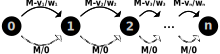
\includegraphics[scale=1.5]{figuras/grafo_rscp_mochila.png}
    \caption{\it Os arcos preenchidos s�o os arcos de $A_1$ e os 
        tracejados de $A_2$. O r�tulo de cada arco $a$ representa $c_a/r_a$.}
    \label{fig:rscp_mochila}
\end{figure}


A constante $M$ pode ser definida como um grande inteiro 
de tal forma que $M-v_i$, para qualquer $i$, seja n�o negativo.
Por quest�o de praticidade, vamos convencionar que representaremos um
arco $(i-1,i) \in A_1$ como $a^1_i$ e um arco $(i-1,i) \in A_2$
como $a^2_i$.

Como $s=0$, $t=n$; podemos ver que qualquer $st$-caminho $P$ 
em $G = (V,A)$ cont�m 
ou $a^1_i$ ou $a^2_i$, $i=1,\dots,n$. Vamos dividir
os arcos de $P$ em dois conjuntos $X$ e $Y$, onde $X$ cont�m os arcos em
$P$ que est�o em $A_1$, e $Y$ cont�m os demais arcos. A partir 
de $X$, vamos definir um subconjunto $S \subseteq N$,
tal que $i \in S$ se e somente se $a^1_i \in X$. 
Com isso,

\begin{equation}
\begin{array}{rcl}
c(P) & = & \displaystyle\sum_{a^1_i \in X}{(M-v_i)} + \displaystyle\sum_{a^2_i \in Y}{M}\\
     & = & n \cdot M - \displaystyle\sum_{a^1_i \in X}{v_i}\\
     & = & n \cdot M - v(S)
\end{array}
\end{equation}

\begin{equation}
\begin{array}{rcl}
r(P) & = & \displaystyle\sum_{a^1_i \in X}{w_i} + \displaystyle\sum_{a^2_i \in Y}{0} \\
     & = & \displaystyle\sum_{a^1_i \in X}{w_i} \\
     & = & w(S)
\end{array}
\end{equation}

Da�, conclu�mos que todo subconjunto $S \subseteq N$ cont�m um $st$-caminho $P$ associado, e 
vice-versa, por meio da equival�ncia 
$i \in S \Leftrightarrow a^1_i \in P$.
Pelas equa��es $(1)$ e $(2)$, um conjunto $S$ e um caminho $P$ associados, 
possuem $r(P)=w(S)$
e $c(P) = n \cdot M - v(S)$. E da� temos dois resultados:
\begin{displaymath}
\begin{array}{rcl}
r(P) \leq l & \Longleftrightarrow & w(S) \le d$$\\
\text{ minimizar } c(P) & \Longleftrightarrow & \text{ maximilizar }v(S)
\end{array}
\end{displaymath}
\end{prova}


